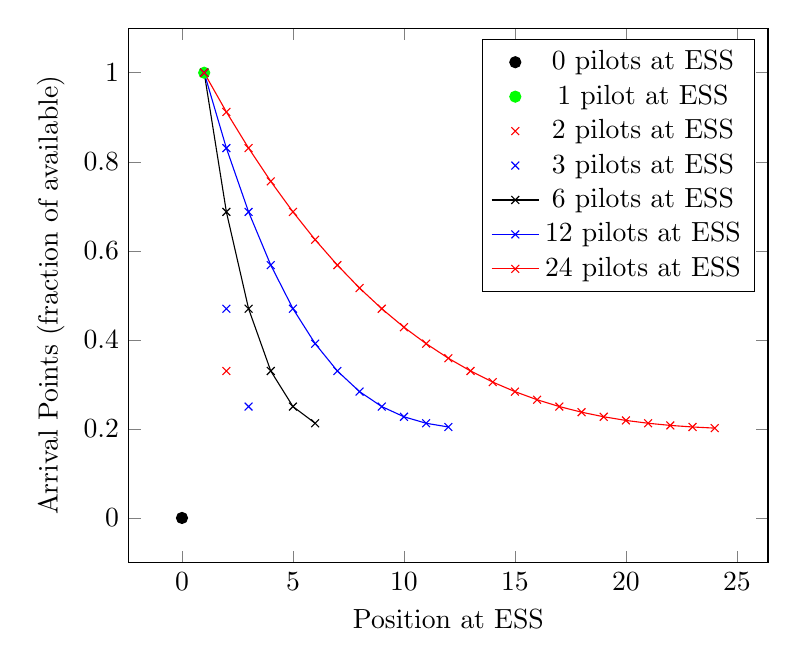
\begin{tikzpicture}
\begin{axis}[ xlabel=Position at ESS
            , ylabel=Arrival Points (fraction of available)
            , width=0.8\textwidth
            ]
    \addplot[ black
            , only marks
            , mark=*
            ] coordinates { (0,0) };
    \addplot[ green
            , only marks
            , mark=*
            ] coordinates { (1, 1) };
    \addplot[ red
            , only marks
            , mark=x
            , domain=1:2
            , samples=2
            ]{0.2 + 0.037*(1 - (x - 1)/2) + 0.13*(1 - (x - 1)/2)^2 + 0.633*(1 - (x - 1)/2)^3};
    \addplot[ blue
            , only marks
            , mark=x
            , domain=2:3
            , samples=2
            ]{0.2 + 0.037*(1 - (x - 1)/3) + 0.13*(1 - (x - 1)/3)^2 + 0.633*(1 - (x - 1)/3)^3};
    \addplot[ black
            , mark=x
            , domain=1:6
            , samples=6
            ]{0.2 + 0.037*(1 - (x - 1)/6) + 0.13*(1 - (x - 1)/6)^2 + 0.633*(1 - (x - 1)/6)^3};
    \addplot[ blue
            , mark=x
            , domain=1:12
            , samples=12
            ]{0.2 + 0.037*(1 - (x - 1)/12) + 0.13*(1 - (x - 1)/12)^2 + 0.633*(1 - (x - 1)/12)^3};
    \addplot[ red
            , mark=x
            , domain=1:24
            , samples=24
            ]{0.2 + 0.037*(1 - (x - 1)/24) + 0.13*(1 - (x - 1)/24)^2 + 0.633*(1 - (x - 1)/24)^3};
    \legend{ 0 pilots at ESS
           , 1 pilot at ESS
           , 2 pilots at ESS
           , 3 pilots at ESS
           , 6 pilots at ESS
           , 12 pilots at ESS
           , 24 pilots at ESS
           }
\end{axis}
\end{tikzpicture}
